\section{Implementierung}
In diesem Kapitel wollen wir auf die Implementierung unseres Prototypen eingehen.


\subsection{Vorstellung des Ablaufs}
Bevor wir auf die konkrete Implementierung eingehen, wollen wir zunächst den grundsätzlichen Ablauf des Prozesses anhand einer Skizze beschreiben:
\begin{figure}[H]
\centering
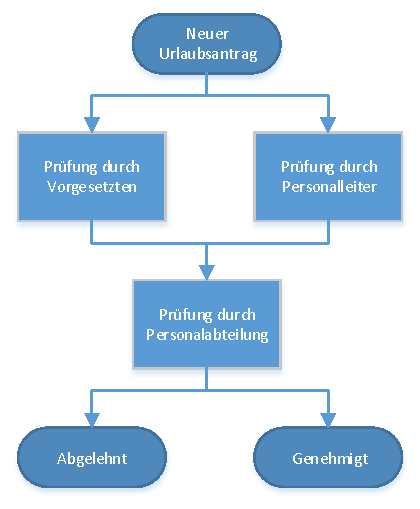
\includegraphics[width=0.5\linewidth]{Bilder/Workflow}
\caption{Skizze des Prozessablaufs}
\label{fig:Workflow}
\end{figure}

Hat ein Mitarbeiter einen Urlaubsantrag ausgefüllt startet ein neuer Urlaubsgenehmigungsprozess. Der Antrag muss an verschiedenen Stellen geprüft werden. In unserem Beispielunternehmen muss der Urlaubsantrag durch den Vorgesetzten und ggf. dem Leiter der Personalabteilung genehmigt werden. Da die Reihenfolge hierbei keine Rolle spielt, können die beiden Schritte parallel ausgeführt werden. Abschließend prüft die Personalabteilung, ob der Mitarbeiter noch über genügend freie Urlaubstage verfügt und genehmigt bzw. verweigert den Antrag.	
	
	
\subsection{Systemübersicht}
	-Überblick verschaffen / Komponenten
		-Datenmodell (Application und Notification)
		-Schnittstellen
		-Workflow
		-GUI (JDialogs und Console)

\subsection{Datenmodell}

\subsection{Schnittstellen}

\subsection{Business Workflow}

\begin{figure}
\centering
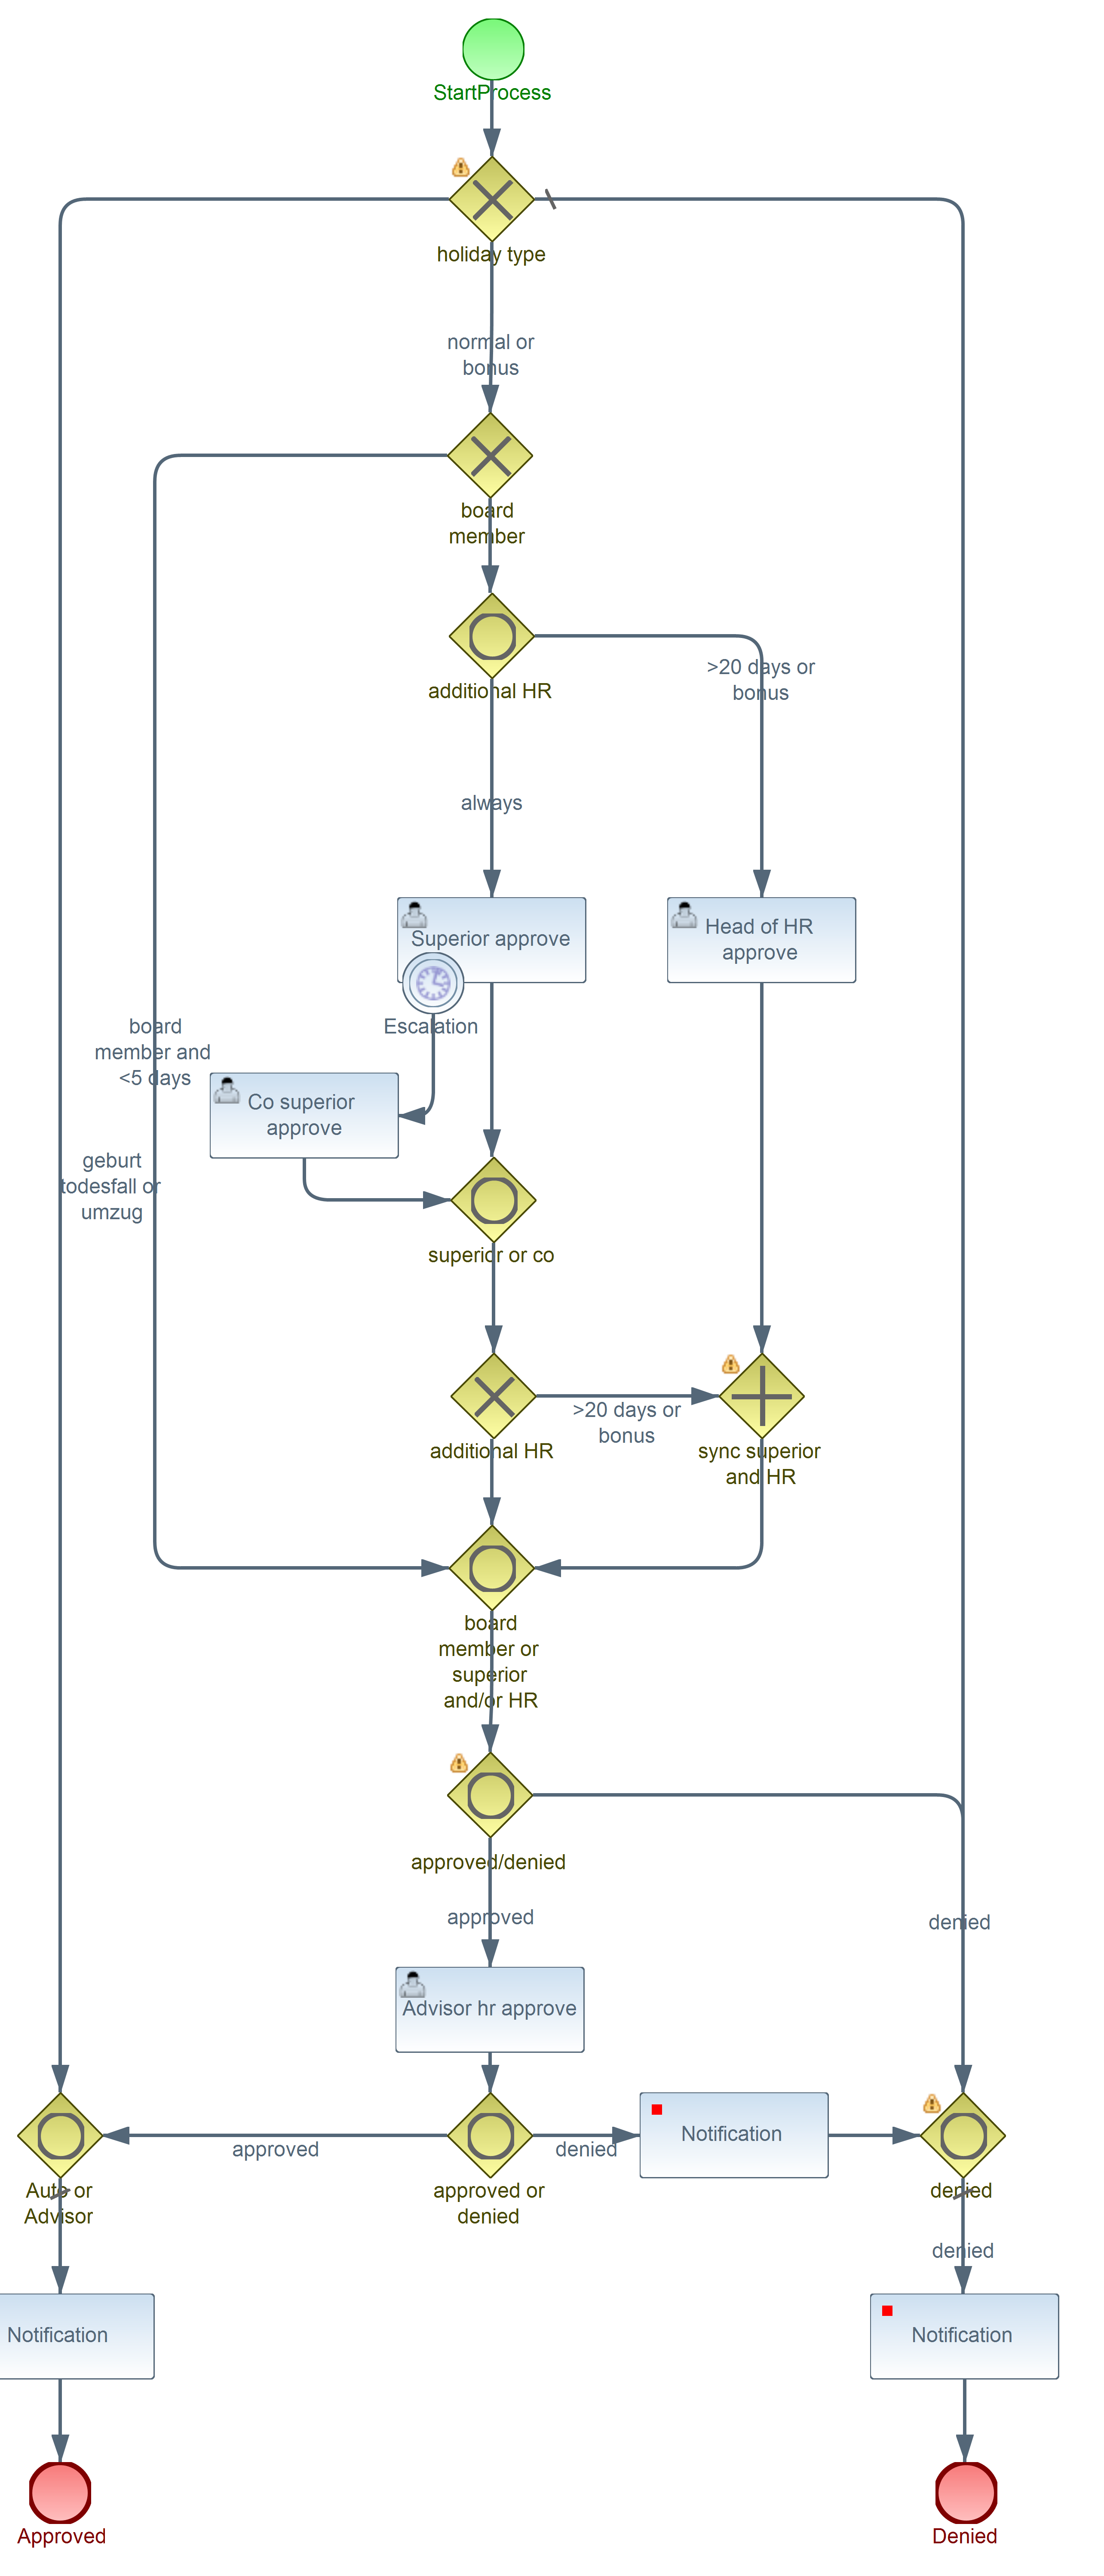
\includegraphics[width=0.7\linewidth]{Bilder/Urlaubsantrag}
\caption{}
\label{fig:Urlaubsantrag}
\end{figure}


\subsection{GUI}